%%%
% Conférence « Comment bien démarrer son projet »
% Vendredi 13 novembre 2009
% Partie « Programmation » par Pierre-Marie de Rodat
%%%

\section{Programmation}

\subsection{Bien architecturer son projet}

\begin{frame}
    \begin{block}{Pourquoi ?}
        \begin{itemize}
            \item Rend plus aisé l'ajout de fonctionnalités
            \item Facilite la recherche et la correction de bugs
            \item Facilite la compréhension du code dans l'équipe
            \item Rend possible le travail en groupe
        \end{itemize}
    \end{block}
\end{frame}


\begin{frame}
    \begin{block}{Comment ?}
        \begin{itemize}
            \item Prendre du recul sur le projet et abstraire les problèmes
            \item Réfléchir avant de coder
            \item Refactoriser en permanence
        \end{itemize}
    \end{block}
\end{frame}

\begin{frame}
  Dressez un descriptif rapide de votre projet.
  \begin{center}
    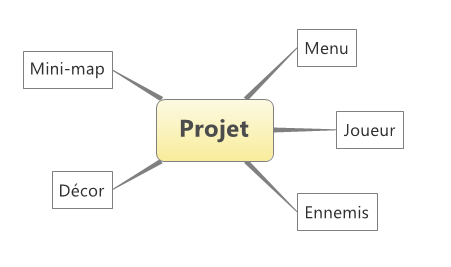
\includegraphics[scale=0.6]{images/project_overview.png}
  \end{center}
\end{frame}

\begin{frame}
  Détaillez les caractéristiques des éléments de votre projet.
    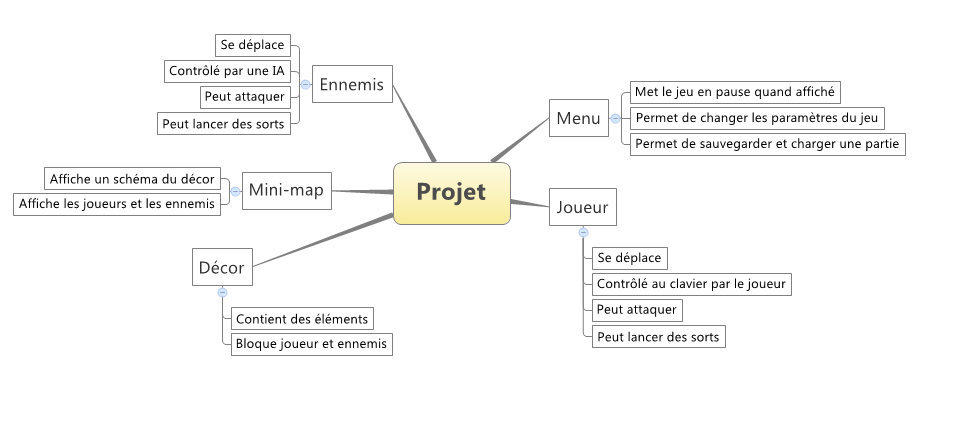
\includegraphics[scale=0.4]{images/project_overview2.png}
\end{frame}

\begin{frame}
  Regroupez les éléments partageant des comportements similaires.
    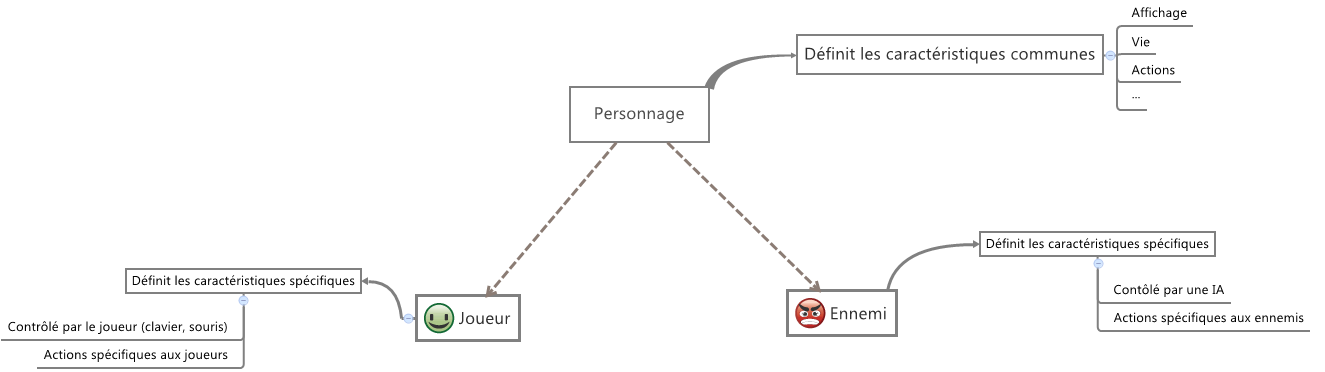
\includegraphics[scale=0.3]{images/project_overview3.png}
\end{frame}
